\documentclass{article}

% Gives us lovely headers
\usepackage{fancyhdr}
% Means you don't have to put \\ to start a new line.
\usepackage[parfill]{parskip}

% For diagrams
\usepackage{tikz}
\usetikzlibrary{shapes, patterns}
\definecolor{light-gray}{gray}{0.95}

\begin{document}
% Meta
\author{Chris Williamson, Todd Davies}
\title{COMP15111 Notes}
\rhead{COMP15111 Notes}

\maketitle
\tableofcontents
\newpage

\section{Lecture 1: Introduction}
\subsection{A Computational Model}
The simplest, earliest, commonest, most important computational model is the \textbf{Von-Neumann Imperative Procedural Computer Model}

According to this model, a computer can:
\begin{enumerate}
	\item Store information
	\item Manipulate the stored information
	\item Make decisions depending on the stored information
\end{enumerate}

\subsection{Simple View Of A Computer}
\[
	Memory \Leftrightarrow Bus \Leftrightarrow Processor
\]

\subsubsection{Memory}
Memory is a set of locations which can hold information, such as numbers(or programs). Each memory location has a unique (numerical) address, and there are typically thousands of millions of different locations. There are various ways of depicting memory; a common one is a 'hex dump' that often looks something like this: \marginpar{\raggedright Run the command {\it hexdump} to generate hexdumps.}

\begin{tabular}{l l l}
	Address     &	Values (8 bit numbers)	&	Characters\\
	00000000	&	48 65 6c 6c 6f 0a		&	Hello.\\
\end{tabular}

Each item that is in the memory has a unique address.

\subsubsection{Bus}
A bus is a bidirectional communication path. It is able to transmit addresses and numbers between components inside the computer.

\subsubsection{Processor}
The processor obeys a sequence of instructions, commonly referred to as a program.
Historically the processor was often referred to as a CPU, however, this is inappropriate nowadays since typical processors consist of several processing cores.

\subsection{Three-address instructions}
Every kind of processor has a different set of instructions, real world examples include: Pentium, ARM and others

Each three-address instruction:
\begin{enumerate}
	\item Copies the values from any two memory locations and sends them to the processor (source operands)
	\item Copies some operation e.g. adds the copied numbers together
	\item Copies the result back from the processor into a third memory location (destination operand)
\end{enumerate}

For example, if we wanted to convert the Java code $sum = a + b;$ into a three-address instruction we would:
\begin{enumerate}
	\item Identify the two {\it source operands}: $a$ holds 2, $b$ holds 3
	\item Perform the {\it operation}: 2 + 3 = 5
	\item Let the variable $sum$ equal the answer 5. This is the {\it destination operand}
\end{enumerate}

\subsubsection{Three address example}
{\bf Question:} Convert the Java code {\it product = c * d;} into the three-address style and draw a two box view of it.

First we need to re-write the Java code in the three-address style:
\[
	product \leftarrow c * d
\]
Now we can draw the box view of it:
\begin{center}
    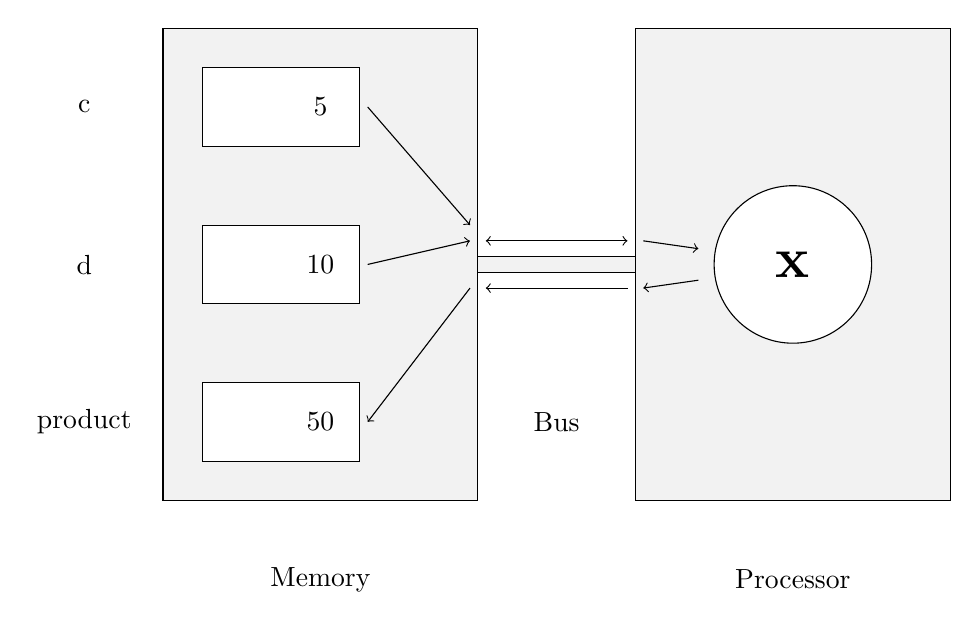
\begin{tikzpicture}
    	% Memory box
    	\draw [fill=light-gray] (-5,  3) rectangle (-1, -3);
    	% Memory label
    	\node at (-3, -4) {Memory};
    	% 5 box
    	\draw [fill=white] (-4.5,  2.5) rectangle (-2.5, 1.5);
    	\node at (-3, 2) {5};
    	% 5 to bus arrow
    	\draw [->] (-2.4, 2) -- (-1.1, 0.5);
    	% c label
    	\node at (-6, 2) {c};
    	% 10 box
    	\draw [fill=white] (-4.5,  0.5) rectangle (-2.5, -0.5);
    	\node at (-3, 0) {10};
    	% 10 to bus arrow
    	\draw [->] (-2.4, 0) -- (-1.1, 0.3);
    	% d label
    	\node at (-6, 0) {d};
    	% 50 box
    	\draw [fill=white] (-4.5,  -1.5) rectangle (-2.5, -2.5);
    	\node at (-3, -2) {50};
    	% Bus to 50 arrow
    	\draw [->] (-1.1, -0.3) -- (-2.4, -2);
    	% product label
    	\node at (-6, -2) {product};
    	% Bus rectangle
    	\draw [fill=light-gray] (-1, 0.1) rectangle (1, -0.1);
    	% Bottom bus arrow
    	\draw [<-] (-0.9, -0.3) -- (0.9, -0.3);
    	% Top bus arrow
    	\draw [<->] (-0.9, 0.3) -- (0.9, 0.3);
    	% Bus label
    	\node at (0, -2) {Bus};
    	% Processor box
		\draw [fill=light-gray] (1,  3) rectangle (5, -3);
		% Bus to processor
    	\draw [->] (1.1, 0.3) -- (1.8, 0.2);
    	% Processor to bus
    	\draw [<-] (1.1, -0.3) -- (1.8, -0.2);
		% Processor label
    	\node at (3, -4) {Processor};
    	% Multiplication circle
    	\draw [fill=white] (3, 0) circle [radius=1];
    	\node at (3, 0) {\huge \bf x};
    \end{tikzpicture}
\end{center}

\subsubsection{Memory bottleneck}
Most processors can process instructions faster than they can be fed by memory. Each instruction in the three-address cycle requires four memory cycles:

\begin{enumerate}
    \item Fetch the instruction
    \item Read the first operand
    \item Read the second operand
    \item Write the result to memory
\end{enumerate}

Each of these memory cycles could take hundreds of processor clock cycles to complete, and so in this time the processor would be doing nothing. However, most modern processors employ a {\it cache} to temporarily store commonly accessed memory locations, and so avoid some of the memory cycles. 

\subsection{Registers}
Registers are very small amounts of storage build into a processor. Since they are inside the processor data doesn't need to be transferred over the bus, and so they are very fast. Registers are used instead of the main memory which speeds up program execution.

Each register can only hold one value and each processor will only generally have a few dozen registers (e.g. ARM has sixteen).

\subsection{Instruction Styles}

\subsubsection{One address}
The one address style can only use up to one memory location in each instruction, all other operands must be registers. An example may be:

\[
    R1 \leftarrow R0 + \textrm{\it memory location}
\]

\subsubsection{Load-store}
The load-store style cannot perform operations on memory locations at all. Instead, values from memory must be loaded into a registers before the operation takes place and then the operation can be performed on the registers. Following the operation, the result must be stored back into memory again.

\[
    R1 \leftarrow \textrm{\it memory location}\\
	R1 \leftarrow R0 + R1\\
    \textrm{\it memory location} \leftarrow R1
\]

This means that we need extra instructions to do stuff with memory locations:
\begin{enumerate}
	\item \textbf{Load} the value from memory into a register before the operation.
	\item \textbf{Store} the value in the register back to memory after the operation.
\end{enumerate}

For example, the Java code {\it Sum = a + b + c;} would be run as:

\begin{center}
    \begin{tabular}{l l l r}
        R1 & $\leftarrow$ & a & (i.e. load from a)\\
        R2 & $\leftarrow$ & b & (i.e. load from b)\\
        R3 & $\leftarrow$ & R1 + R2 & (i.e. a+b)\\
        R4 & $\leftarrow$ & c & (i.e. load from c)\\
        R5 & $\leftarrow$ & R3 + R4  & (i.e. (a+b)+c)\\
        Sum & $\rightarrow$ & R5 & (i.e. store to sum)\\
    \end{tabular}
\end{center}

You can see that the load-store style favours lots of very simple, very fast instructions.

\section{Lecture 2}
Computers obey programs which are sequences of instructions. Instructions are coded as values in memory. The sequences are held in memory adjacent memory locations. Values in memory can be interpreted as you please, from numbers to text, to images or anything really!

Any given set of binary digits can be read as a decimal number, but not always as text, so values in memory are often represented as numbers for convenience.

\subsection{Assembly Language}
Assembly language is a means of representing machine instructions in a human readable form.

Each type of processor has its own assembly language (since each language is specific to a partial architecture) but they typically have a lot in common:

\begin{itemize}
	\item A mnemonic, that specifies the type of operation
	\item A destination, such as a register or memory location
	\item And one or more sources that may be registers or memory locations.
	\item Possibly with a comment too which will help programmers understand what's happening and aren't interpreted by the assembler.
\end{itemize}

When a program has been written in assembler, it must be {\it assembled} by an {\it assembler} to run it.

\subsection{ARM instructions}

ARM has many instructions but we only need three categories:

\begin{itemize}
	\item Memory operations that move data between the memory and the registers.
	\item Processing operations that perform calculations using value already in registers.
	\item Control flow instructions are used to make decisions, repeat operations etc.
\end{itemize}

\subsection{Transferring data between registers and memory}

Memory operations load a register from the memory or store a register value to the memory.

For example, $a$ into register 1 ($R1 \leftarrow a$) we would write:
{\tt LDR R1, a}

Or to store the value in register 5 into $sum$ ($sum \leftarrow R5$):
{\tt STR R5, sum}

In these examples, $a$ and $sum$ are aliases for the addresses of memory locations.

\subsection{ARM processing instructions}
Processing operations such as addition, subtraction, multiplication.

e.g. ADD R3, R1, R2 – means: R3 \(\leftarrow\) R1 + R2

\subsection{ARM control instructions}
Fundamentally, these are branches to other code sequences. Often, branches are made conditional to allow decisions to be made.

% TODO: Clean this into a math/code/tabular environment or something.
e.g. B somewhere – means: branch to ‘somewhere’\\
e.g. BEQ elsewhere – means: branch to ‘elsewhere’ IF ‘previous result’ was ‘equals’\\
e.g. BNE wherever – means: branch to ‘wherever’ IF ‘previous result’ was ‘not equal’\\

\subsection{Stored programs and the Program Counter}
A computer can make decisions, and choose which instructions to obey next depending upon the results of those decisions. How? First we need to see how the sequence of instructions is controlled. Von-Neumann Model: memory holds both instructions and numbers - \textbf{stored program} \textbf{Program Counter} (PC) register: holds the address of the memory location containing the next instruction to b obeyed (executed).

ARM uses register 15 as its PC

\subsection{Fetch-Execute Cycle}
Start with PC containing the address of (the memory location holding) the first instruction of a program.

Repeatedly:
\begin{enumerate}
	\item \textbf{Fetch}: copy the instruction, pointed to by the PC, from memory and set PC to point to the next instruction
	\item \textbf{Execute}:  obey the instruction (exactly as before)
\end{enumerate}
ARM:
\begin{enumerate}
	\item 'Resets' to (starts at) address 00000000
	\item Instructions each occupy 4 memory locations, so PC increases by 4 in each fetch
\end{enumerate}

\subsection{Decision Making}
Linear sequences of instructions are limiting. To make a decision, the computer must change (or not) to a
different sequence of instructions.

e.g. a 1 pound discount on items worth 20 pounds or more.
Decision: compare the total and 20 pounds to see if it is larger, then depending on result, either perform action or not.
Action: subtract 1 pound from the total.\\

Computers have no intelligence, so spell out details.
\textbf{Formalise}: if total \(\geq\) 20 pounds then subtract 1 pound from total\\
\textbf{Rewrite}: if total \(\textless\) 20 pounds then don’t\\
\textbf{subtract} 1 pound from total\\
Encode: as ARM instructions

\subsection{Compare And Branch}

\end{document}

